\subsection{Data Visualization}

Phần này trình bày trực quan hoá hành vi giá, thanh khoản, độ biến động và phân phối lợi suất của 10 đồng coin trong Kho dữ liệu (BTC, ETH, BNB, SOL, XRP, ADA, DOGE, TRX, DOT, MATIC). Tất cả các biểu đồ được sinh trực tiếp từ \texttt{gold.fact\_market\_daily} thông qua script \texttt{tools/generate\_report\_images.py} sử dụng các thư viện chuẩn \texttt{matplotlib} và \texttt{seaborn} \cite{mckinney2017}.

\subsubsection{Biểu đồ giá đóng cửa của từng coin}

\paragraph{Bitcoin (BTC) -- ``vàng kỹ thuật số''}
\begin{figure}[H]
    \centering
    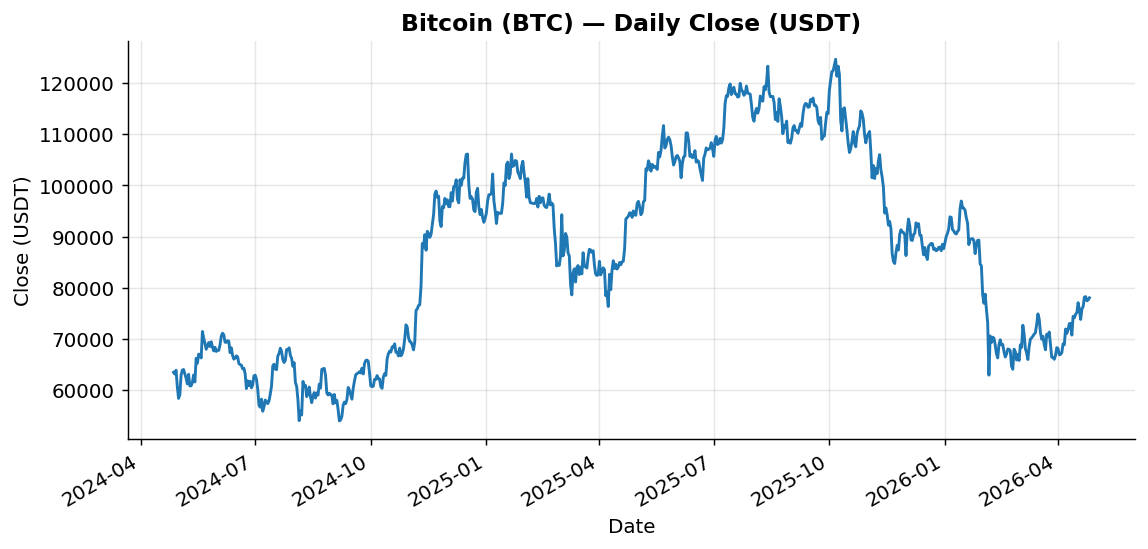
\includegraphics[width=0.85\textwidth]{Images/visualization/BTC_close_chart.png}
    \caption{Diễn biến giá đóng cửa của BTC (USDT)}
    \label{fig:btc_close}
\end{figure}
Biểu đồ \ref{fig:btc_close} cho thấy BTC trải qua chu kỳ tăng trưởng mạnh sau Halving (04/2024), bứt phá vùng đỉnh cũ và lập đỉnh lịch sử mới. Sau giai đoạn phấn khích này là một pha điều chỉnh sâu (drawdown $\sim$50\%) trước khi ổn định lại. Đặc trưng của BTC: \emph{biến động lớn nhưng có tính chu kỳ rõ rệt}, là đại diện ``low-vol'' trong nhóm coin (so với altcoin còn lại) và đóng vai trò ``tài sản trú ẩn'' trong các giai đoạn rủi ro cao.

\paragraph{Ethereum (ETH) -- nền tảng smart contract dẫn đầu}
\begin{figure}[H]
    \centering
    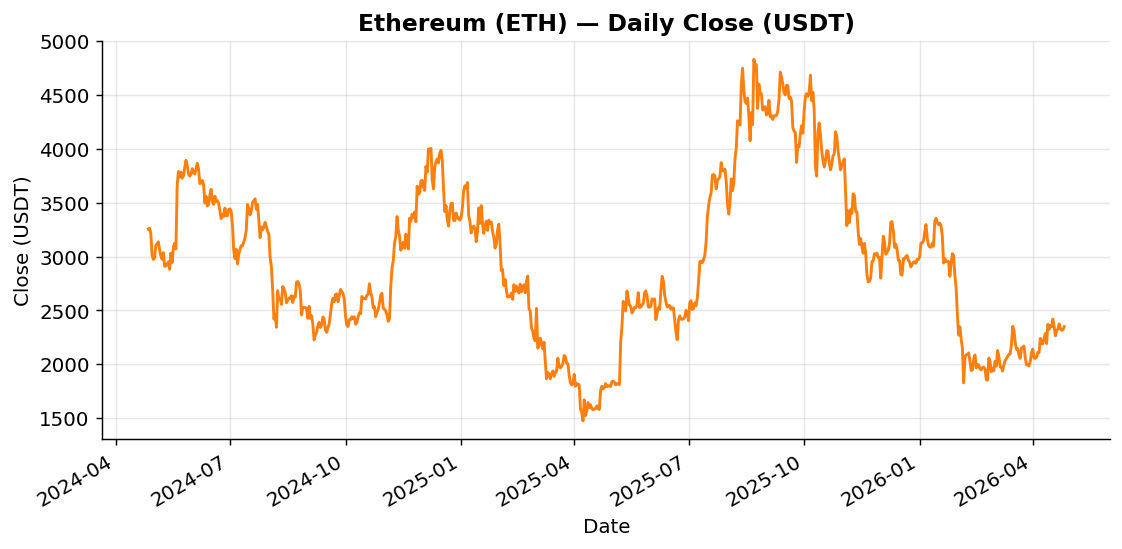
\includegraphics[width=0.85\textwidth]{Images/visualization/ETH_close_chart.png}
    \caption{Diễn biến giá đóng cửa của ETH (USDT)}
    \label{fig:eth_close}
\end{figure}
Biểu đồ \ref{fig:eth_close} cho thấy ETH có hiệu suất kém hơn BTC trong giai đoạn này: pha tăng trưởng yếu, drawdown tới $\sim$63\% từ đỉnh. Lý do chính là sự cạnh tranh từ các Layer-1 đối thủ (SOL) và sự hấp dẫn dòng tiền vào BTC ETF.

\paragraph{Solana (SOL) -- ``ETH killer'' với độ biến động cao}
\begin{figure}[H]
    \centering
    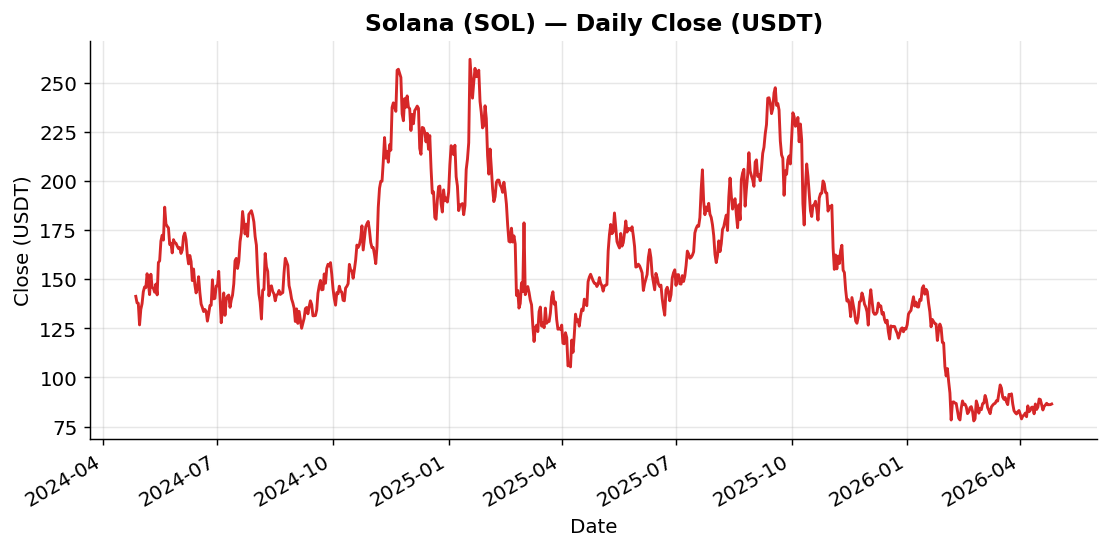
\includegraphics[width=0.85\textwidth]{Images/visualization/SOL_close_chart.png}
    \caption{Diễn biến giá đóng cửa của SOL (USDT)}
    \label{fig:sol_close}
\end{figure}
SOL (hình \ref{fig:sol_close}) là minh chứng cho ``high risk -- high reward''. Cú tăng vượt bậc cuối 2024 (theo đà meme coin trên hệ Solana) đi kèm drawdown $\sim$70\% sau khi pha hype kết thúc.

\paragraph{XRP -- biến động kiểu sự kiện (event-driven)}
\begin{figure}[H]
    \centering
    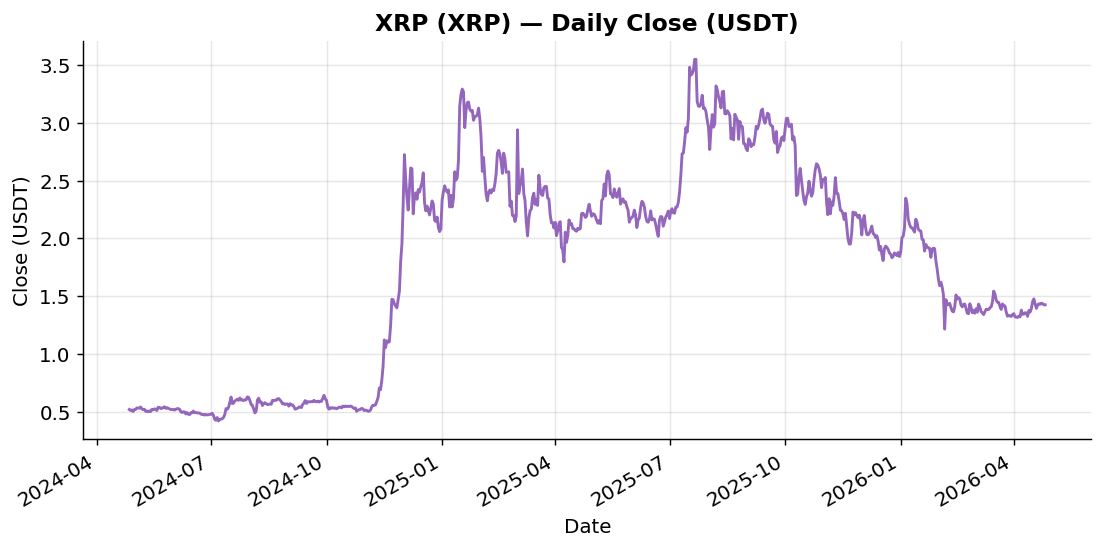
\includegraphics[width=0.85\textwidth]{Images/visualization/XRP_close_chart.png}
    \caption{Diễn biến giá đóng cửa của XRP (USDT)}
    \label{fig:xrp_close}
\end{figure}
XRP (hình \ref{fig:xrp_close}) thể hiện rõ kiểu biến động ``event-driven'': giá đi ngang trong nhiều tháng, sau đó bùng nổ rất nhanh khi có tin tức (vụ kiện SEC, ETF). Pha tăng vọt cuối 2024 đưa XRP lên top coin có lợi suất tích luỹ cao nhất trong nhóm phân tích.

\paragraph{DOGE -- meme coin điển hình}
\begin{figure}[H]
    \centering
    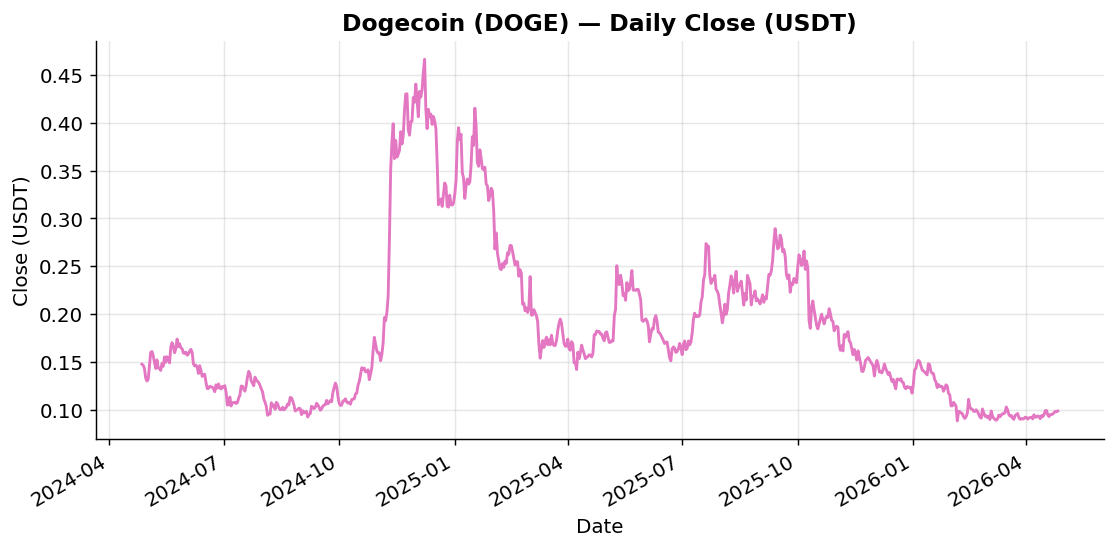
\includegraphics[width=0.85\textwidth]{Images/visualization/DOGE_close_chart.png}
    \caption{Diễn biến giá đóng cửa của DOGE (USDT)}
    \label{fig:doge_close}
\end{figure}
DOGE (hình \ref{fig:doge_close}) là đại diện cho nhóm \texttt{Meme} với \texttt{risk\_level = High}. Biên độ biến động cực lớn, drawdown lên tới $\sim$81\% từ đỉnh -- minh hoạ rõ rủi ro tail của các coin có yếu tố ``meme''.

\paragraph{Cardano (ADA), Polkadot (DOT), Polygon (MATIC) -- các altcoin underperformer}
\begin{figure}[H]
    \centering
    \begin{minipage}{0.49\textwidth}
        \centering
        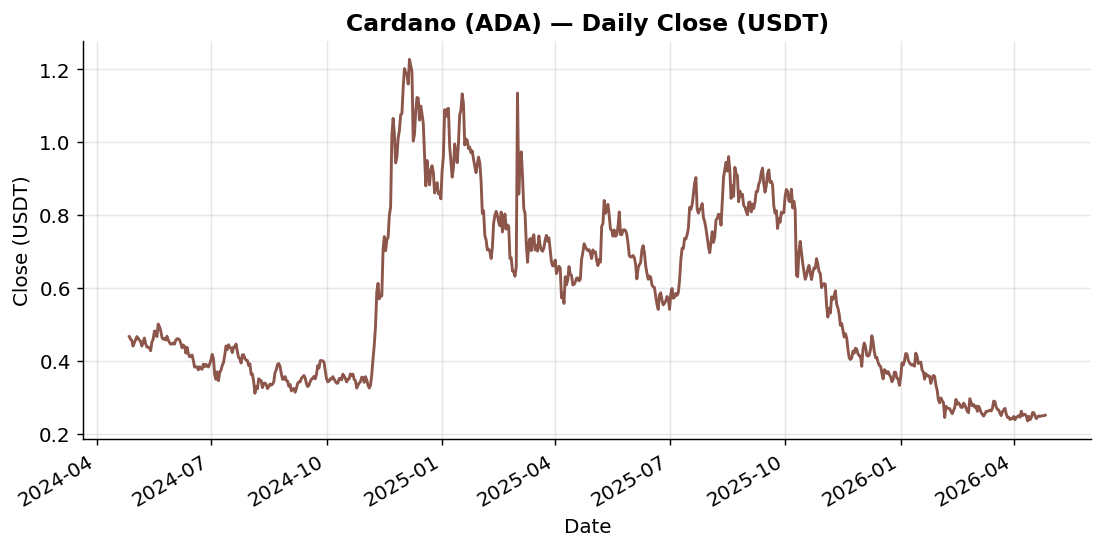
\includegraphics[width=\linewidth]{Images/visualization/ADA_close_chart.png}
        \subcaption{ADA -- drawdown $\sim$80\%}
    \end{minipage}
    \begin{minipage}{0.49\textwidth}
        \centering
        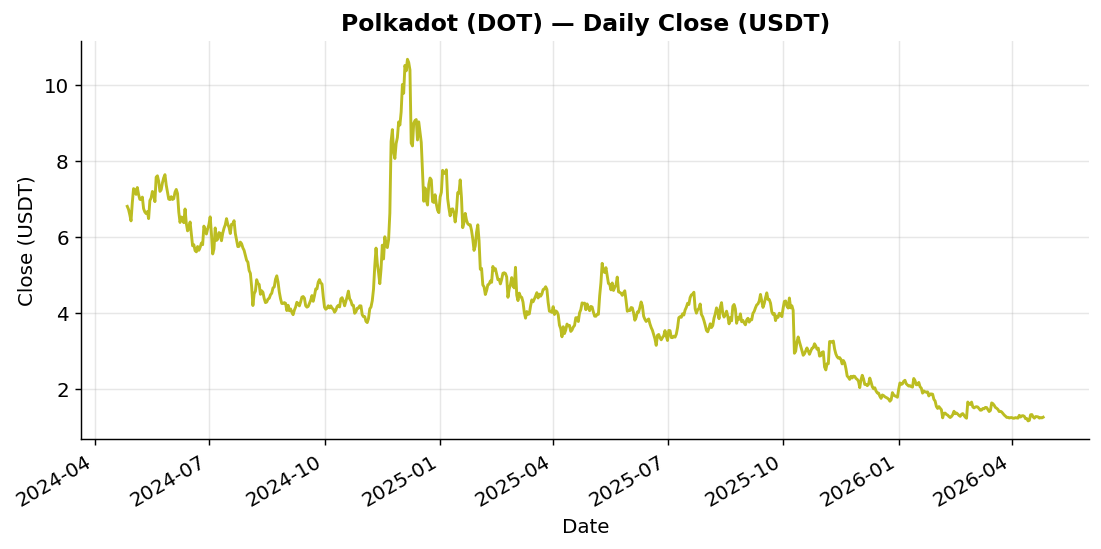
\includegraphics[width=\linewidth]{Images/visualization/DOT_close_chart.png}
        \subcaption{DOT -- drawdown $\sim$89\%}
    \end{minipage}
    \\[6pt]
    \begin{minipage}{0.6\textwidth}
        \centering
        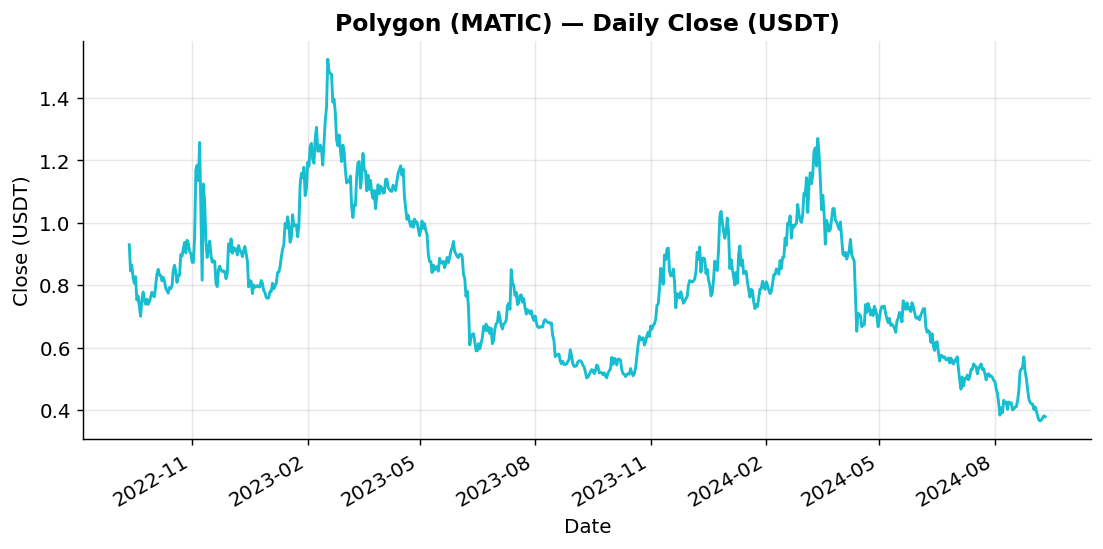
\includegraphics[width=\linewidth]{Images/visualization/MATIC_close_chart.png}
        \subcaption{MATIC -- delist 09/2024 sau khi rebrand POL}
    \end{minipage}
    \caption{Nhóm underperformer: ADA, DOT, MATIC}
    \label{fig:underperformer}
\end{figure}
Cả ba mã (hình \ref{fig:underperformer}) đều rơi vào downtrend kéo dài. ADA và DOT mất 80--89\% giá trị từ đỉnh; MATIC bị Binance delist sau rebrand POL nên dữ liệu chỉ kéo dài đến 09/2024. Đây là nhóm cần thận trọng nhất trong phân bổ danh mục.

\paragraph{BNB, TRX -- nhóm low-vol ổn định}
\begin{figure}[H]
    \centering
    \begin{minipage}{0.49\textwidth}
        \centering
        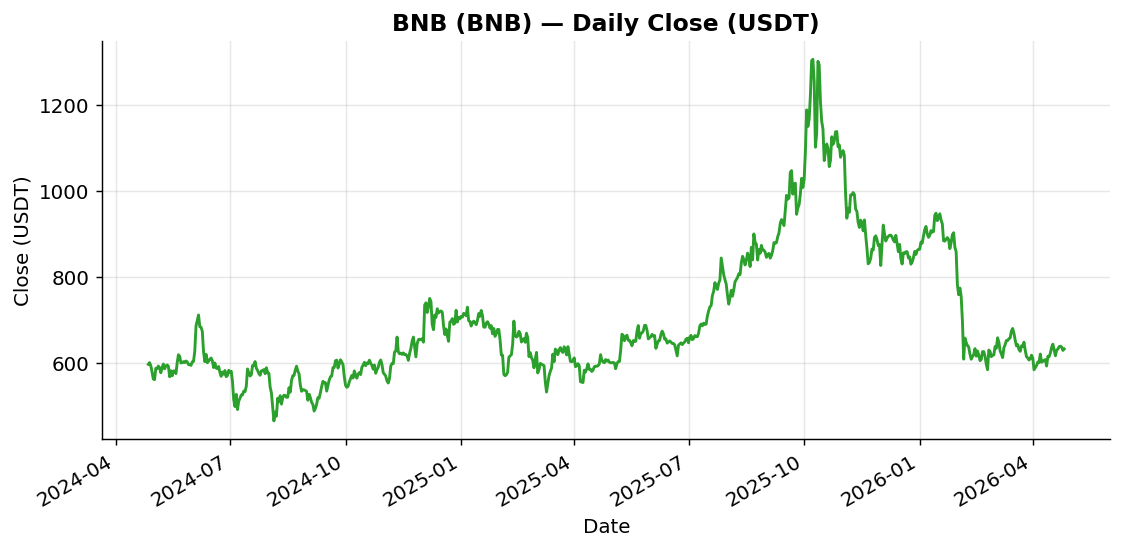
\includegraphics[width=\linewidth]{Images/visualization/BNB_close_chart.png}
        \subcaption{BNB}
    \end{minipage}
    \begin{minipage}{0.49\textwidth}
        \centering
        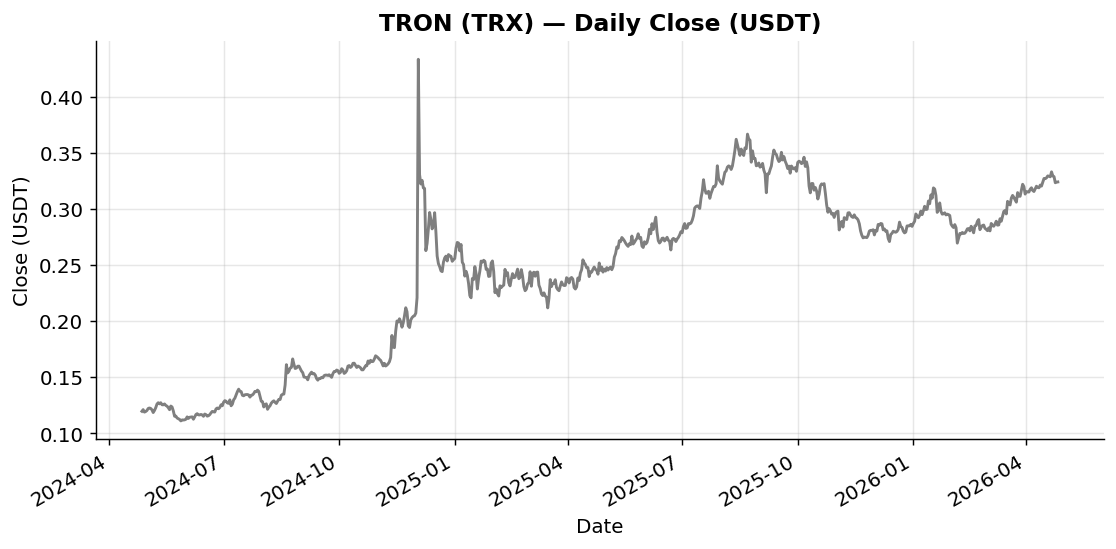
\includegraphics[width=\linewidth]{Images/visualization/TRX_close_chart.png}
        \subcaption{TRX}
    \end{minipage}
    \caption{Nhóm low-vol: BNB, TRX}
    \label{fig:lowvol_pair}
\end{figure}
BNB và TRX (hình \ref{fig:lowvol_pair}) duy trì xu hướng tăng tương đối ổn định, biến động thấp nhất trong nhóm 10 coin. TRX đặc biệt nổi bật với lợi suất trung bình ngày dương rõ rệt và drawdown chỉ $\sim$51\% -- thấp nhất trong nhóm altcoin.

\subsubsection{Biểu đồ so sánh khối lượng giao dịch trung bình các coin}

\begin{figure}[H]
    \centering
    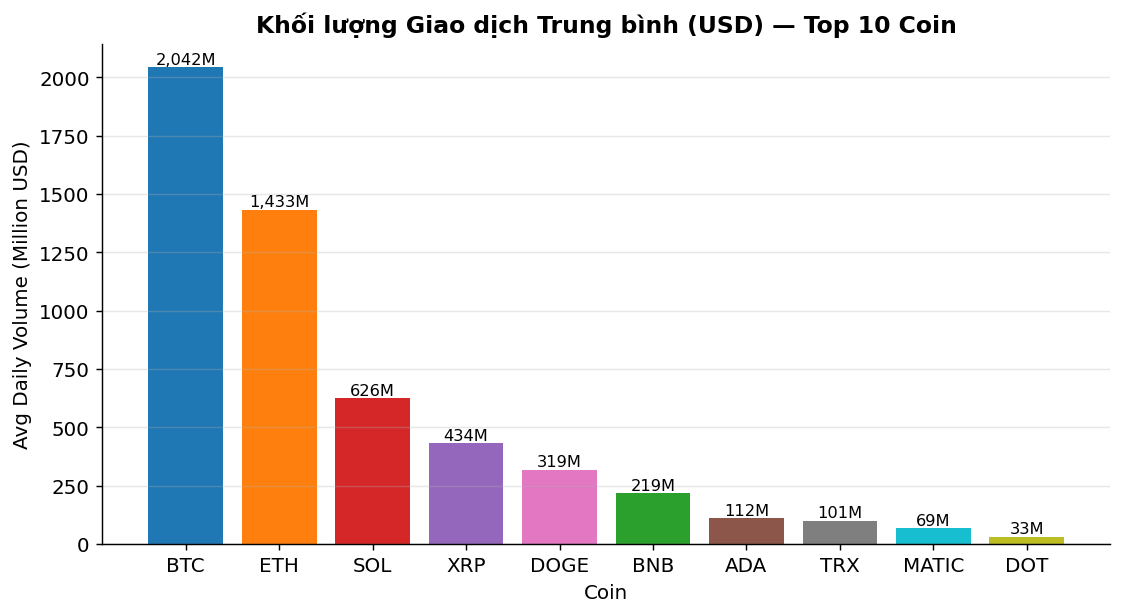
\includegraphics[width=\linewidth]{Images/visualization/AverageVolumn.png}
    \caption{Khối lượng giao dịch trung bình hằng ngày (Million USD)}
    \label{fig:avg_volume}
\end{figure}

Biểu đồ \ref{fig:avg_volume} cho thấy sự phân cực thanh khoản cực mạnh giữa 10 coin:
\begin{itemize}
    \item \textbf{Nhóm 1 -- Thanh khoản vượt trội:} BTC và ETH áp đảo, khối lượng giao dịch trung bình hàng ngày lên tới hàng tỷ USD.
    \item \textbf{Nhóm 2 -- Thanh khoản tốt:} SOL, XRP, DOGE, BNB ở mức hàng trăm triệu USD.
    \item \textbf{Nhóm 3 -- Thanh khoản thấp:} ADA, TRX, DOT, MATIC -- thanh khoản tương đối hạn chế so với nhóm dẫn đầu.
\end{itemize}

Hệ luận quan trọng:
\begin{itemize}
    \item \emph{Tín hiệu giá có độ tin cậy khác nhau giữa các nhóm.} Một breakout trên BTC/ETH với volume spike đáng tin cậy hơn nhiều so với một biến động cùng biên độ trên DOT/MATIC.
    \item \emph{Cần chuẩn hoá khi gom cụm.} Sự chênh lệch volume giữa BTC ($\sim$10$^{10}$) và DOT/MATIC ($\sim$10$^7$) là 3 bậc magnitude, nên K-Means buộc phải qua \texttt{StandardScaler} hoặc dùng \texttt{log10(volume\_usd)} để tránh thiên lệch.
\end{itemize}

\subsubsection{Biểu đồ so sánh hiệu suất đầu tư (Cumulative Growth)}

\begin{figure}[H]
    \centering
    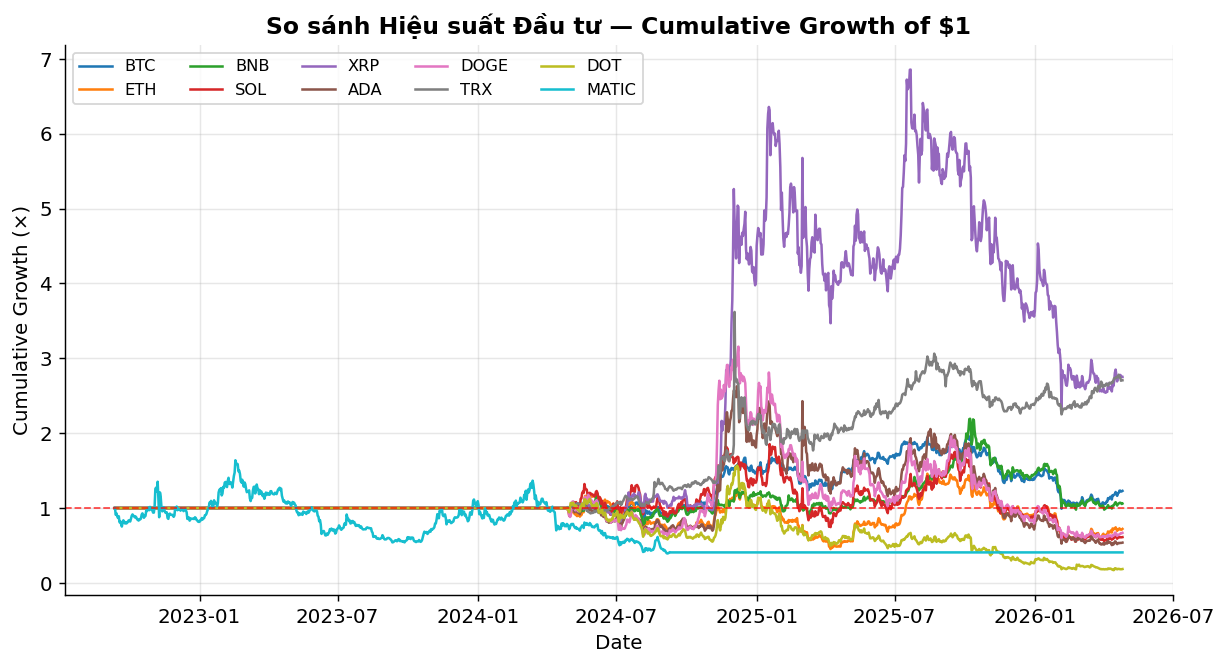
\includegraphics[width=\linewidth]{Images/visualization/CumulativeLogReturn.png}
    \caption{So sánh hiệu suất đầu tư -- Cumulative Growth của \$1 đầu kỳ}
    \label{fig:cum_return}
\end{figure}

Biểu đồ \ref{fig:cum_return} chuẩn hoá giá trị của tất cả 10 coin về mức 1.0 vào đầu kỳ (27/04/2024). Đường biểu diễn cho thấy giá trị của \$1 đầu tư ban đầu sẽ thay đổi như thế nào theo thời gian:

\begin{itemize}
    \item \textbf{Outperformer -- XRP, TRX, BTC:} Có lợi suất trung bình ngày dương rõ rệt, kết thúc kỳ với mức tăng trưởng vượt trội. XRP đặc biệt nổi bật với cú bứt phá cuối 2024.
    \item \textbf{Trung tính -- BNB:} Lợi suất trung bình ngày gần 0, đường cumulative growth dao động quanh mức 1.0.
    \item \textbf{Underperformer -- ETH, SOL, DOGE:} Sau pha tăng đầu kỳ, đều rơi vào downtrend, kết thúc dưới mức 1.0.
    \item \textbf{Lỗ nặng -- ADA, DOT, MATIC:} Mất 50--80\% giá trị, đại diện cho nhóm rủi ro cao nhưng không có phần thưởng tương xứng trong giai đoạn này.
\end{itemize}

Khi kết hợp với biểu đồ thanh khoản (\ref{fig:avg_volume}), các cụm hiển hiện rõ:
\begin{itemize}
    \item Cụm 1 (High Return + High Volume): BTC, XRP
    \item Cụm 2 (Low Return + High Volume): ETH, SOL
    \item Cụm 3 (Stable + Low/Mid Volume): BNB, TRX
    \item Cụm 4 (Negative Return + Low Volume): ADA, DOT, MATIC, DOGE
\end{itemize}

\subsubsection{Biểu đồ biến động trượt (Rolling Volatility)}

\begin{figure}[H]
    \centering
    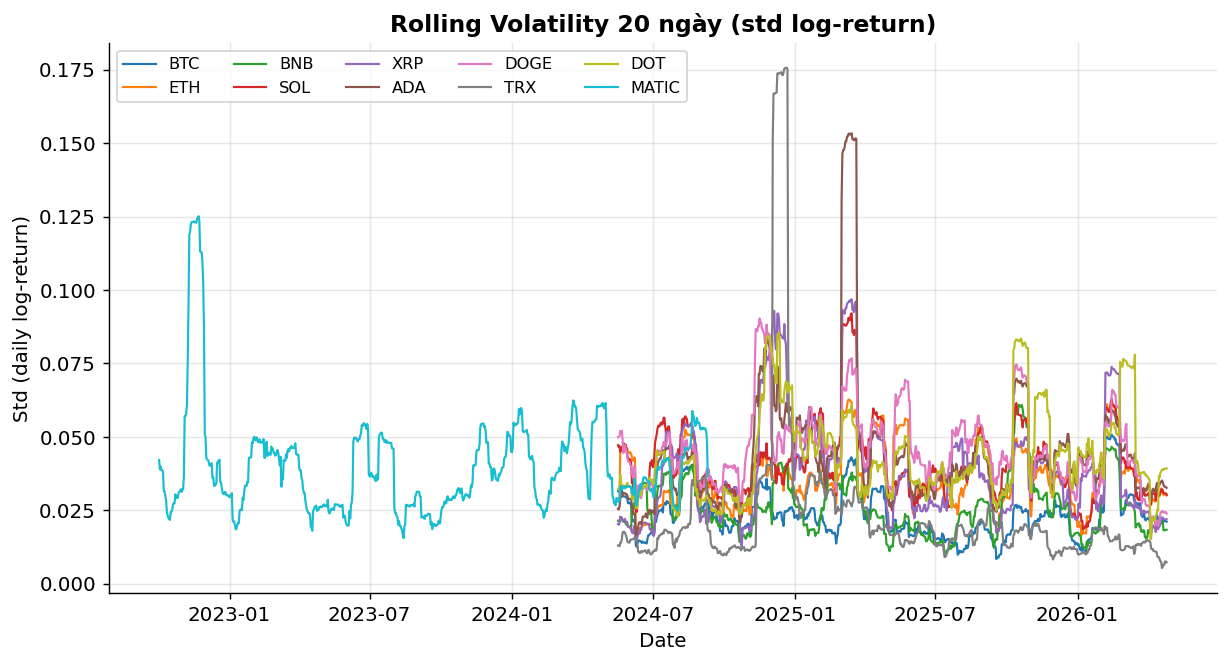
\includegraphics[width=0.85\linewidth]{Images/visualization/RollingVolatility20.png}
    \caption{Mức độ biến động giá -- std log-return cửa sổ 20 ngày}
    \label{fig:rolling_vol_20}
\end{figure}

Biểu đồ \ref{fig:rolling_vol_20} thể hiện độ lệch chuẩn của log-return trên cửa sổ trượt 20 ngày, đo lường rủi ro ngắn hạn của từng coin:

\begin{itemize}
    \item \textbf{Volatility Clustering:} Hiện tượng ``rủi ro tụ lại'' rất rõ -- khi một coin bắt đầu biến động mạnh, nó có xu hướng duy trì trạng thái rủi ro cao trong nhiều tuần (ví dụ giai đoạn cuối Q1/2025 cả thị trường cùng biến động mạnh).
    \item \textbf{Phân nhóm khẩu vị rủi ro:}
    \begin{itemize}
        \item \emph{Rủi ro cao thường trực:} ADA, DOGE, DOT, SOL gần như luôn nằm ở nửa trên biểu đồ với std hằng ngày 4--5\%.
        \item \emph{Rủi ro thấp ổn định:} BTC, BNB, TRX có std hằng ngày chủ yếu 2--3\%, nửa thấp hơn nhóm còn lại.
        \item \emph{Rủi ro thay đổi theo sự kiện:} XRP có giai đoạn biến động cực cao quanh các sự kiện kiện tụng/ETF, sau đó trở lại mức trung bình.
    \end{itemize}
\end{itemize}

\begin{figure}[H]
    \centering
    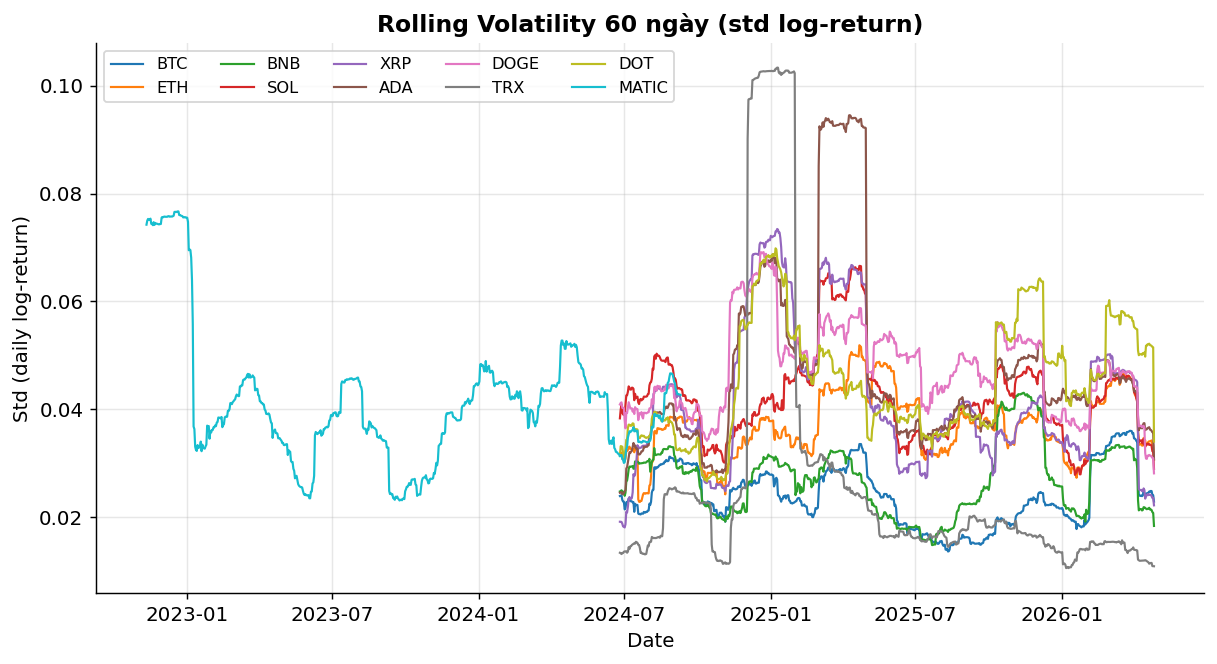
\includegraphics[width=0.85\linewidth]{Images/visualization/RollingVolatility60.png}
    \caption{Mức độ biến động giá -- std log-return cửa sổ 60 ngày}
    \label{fig:rolling_vol_60}
\end{figure}

Biểu đồ \ref{fig:rolling_vol_60} dùng cửa sổ trượt 60 ngày, loại bỏ nhiễu ngắn hạn để thể hiện cấu trúc rủi ro dài hạn:
\begin{itemize}
    \item Nhóm nền tảng (BTC, BNB, TRX) có đường biểu diễn ổn định ở vùng thấp -- xác nhận đặc tính ``low structural risk''.
    \item Nhóm altcoin biến động cao (ADA, DOGE, DOT) duy trì đường biểu diễn ở vùng cao trong hầu hết kỳ.
\end{itemize}

Đây là feature quan trọng cho việc gom cụm bằng K-Means -- thay vì dùng volatility 20 ngày dễ bị nhiễu, dùng volatility 60 ngày giúp K-Means nhận diện chính xác hơn các nhóm có đặc tính rủi ro tương đồng.

\subsubsection{Biểu đồ so sánh phân phối lợi nhuận giữa các coin}

\begin{figure}[H]
    \centering
    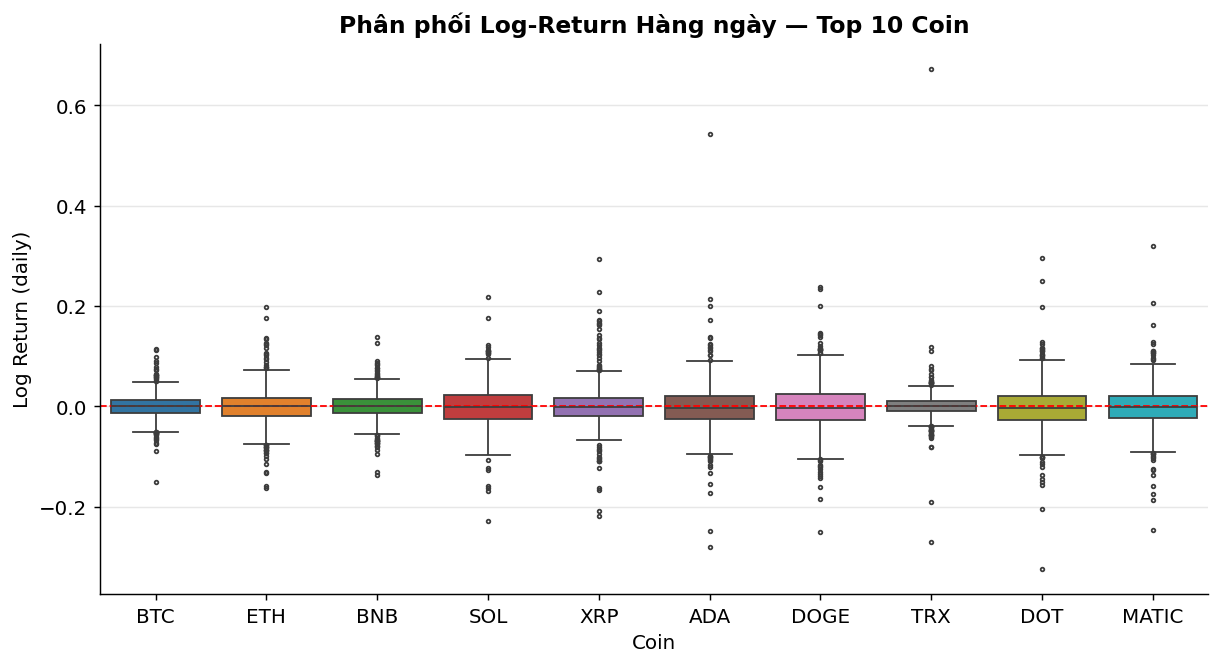
\includegraphics[width=\linewidth]{Images/visualization/boxplot_rui_ro.png}
    \caption{Phân phối log-return hằng ngày của 10 coin}
    \label{fig:boxplot}
\end{figure}

Biểu đồ \ref{fig:boxplot} thể hiện phân phối log-return hằng ngày. Mỗi hộp (box) chứa 50\% số ngày giao dịch điển hình; các chấm tròn ngoài râu (whisker) là các phiên \emph{outlier} cần được phát hiện bằng Anomaly Detection.

\begin{itemize}
    \item \textbf{Trung vị -- hiệu suất kỳ vọng:} XRP và TRX có median dương rõ rệt; BTC, BNB gần 0; ETH, SOL, ADA, DOT, MATIC có median âm.
    \item \textbf{Độ rộng hộp -- biến động:} ADA, DOGE, SOL có hộp rộng nhất, là nhóm rủi ro cao. BTC, BNB, TRX có hộp hẹp nhất.
    \item \textbf{Outlier:} Tất cả coin đều có outlier đối xứng cả hai phía, nhưng DOGE và XRP có nhiều outlier nhất, phù hợp với đặc tính ``event-driven''.
\end{itemize}

\subsubsection{Biểu đồ phân tích đột biến khối lượng (Volume Spike)}

\begin{figure}[H]
    \centering
    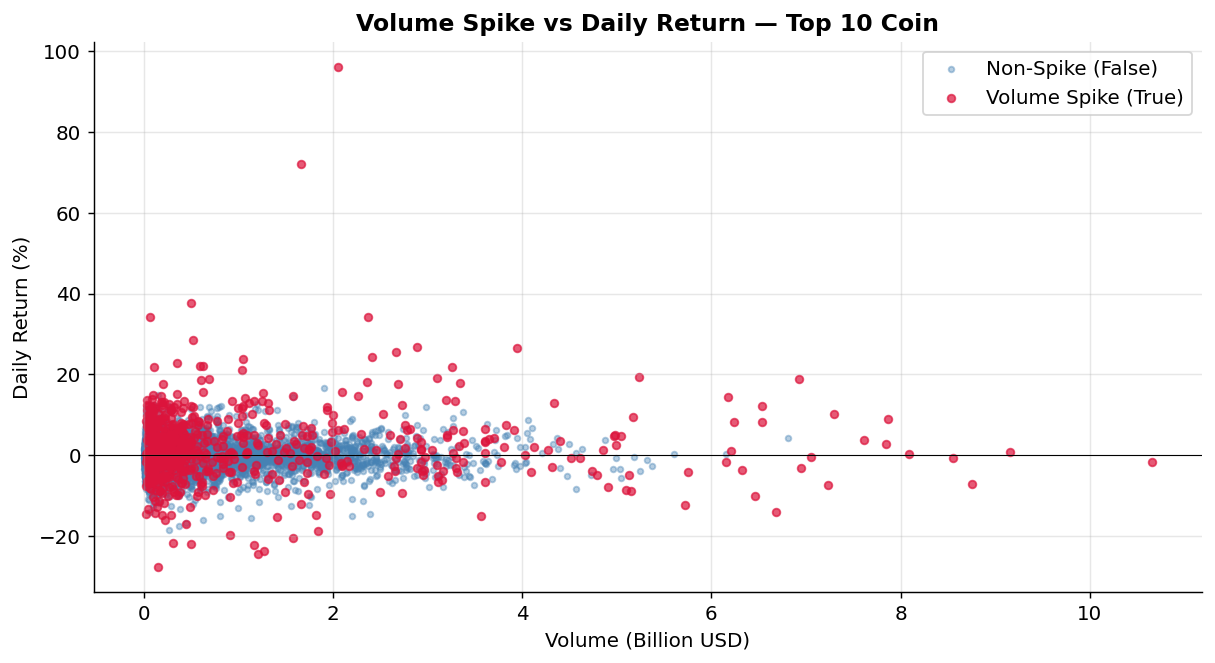
\includegraphics[width=\linewidth]{Images/visualization/VolumeSpikeVsReturn.png}
    \caption{Volume Spike vs Daily Return}
    \label{fig:volume_spike_scatter}
\end{figure}

Biểu đồ \ref{fig:volume_spike_scatter} thể hiện mối quan hệ giữa khối lượng giao dịch (trục X, đơn vị tỷ USD) và lợi nhuận \% (trục Y). Một phiên được đánh dấu là Volume Spike (chấm đỏ) khi \texttt{volume\_usd > 2 $\times$ rolling\_median\_20d}.

\begin{itemize}
    \item \textbf{Phiên thường (xanh):} Tập trung ở phía trái với volume thấp và return dao động hẹp ($\pm$5\%) -- trạng thái cân bằng của thị trường.
    \item \textbf{Phiên Volume Spike (đỏ):} Phân bố ở phía phải, lệch về biên trên hoặc biên dưới của trục Y. Ít phiên Spike kết thúc với return $\sim$0.
\end{itemize}

Điều này khẳng định: \emph{volume bùng nổ là tín hiệu rõ của biến động giá lớn, theo cả hai chiều.}

\begin{figure}[H]
    \centering
    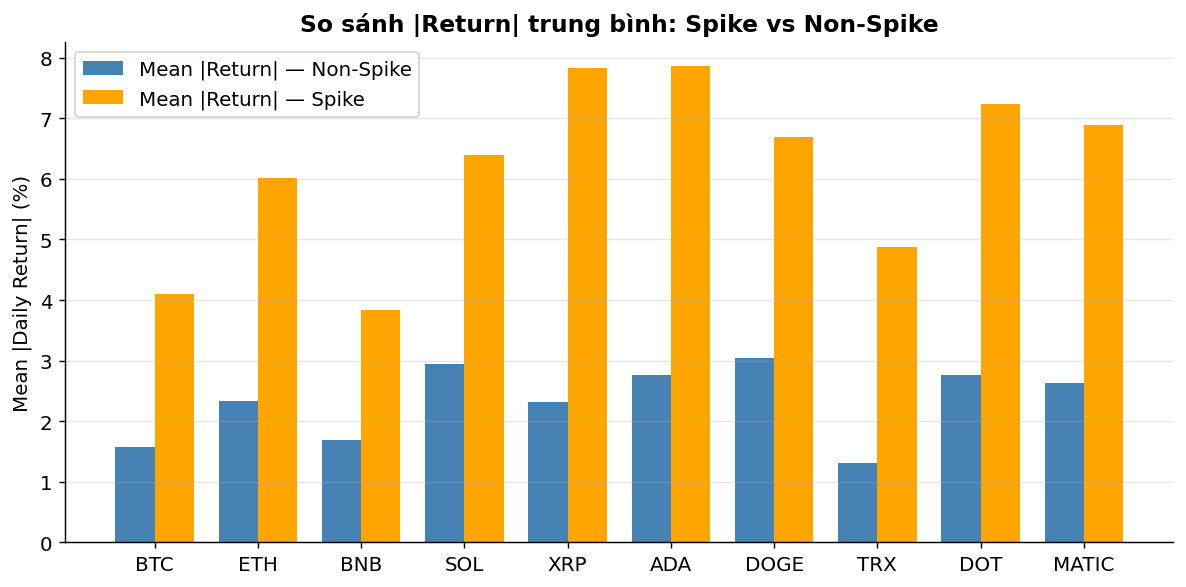
\includegraphics[width=0.85\linewidth]{Images/visualization/SpikeVsNon-Spike.png}
    \caption{So sánh $|Return|$ trung bình: Spike vs Non-Spike}
    \label{fig:spike_vs_nonspike}
\end{figure}

Biểu đồ \ref{fig:spike_vs_nonspike} là kết luận định lượng: với mọi coin, cột màu cam ($|Return|$ trong ngày Spike) luôn cao gấp \textbf{2--3 lần} cột xanh (Non-Spike). Mối quan hệ này phổ quát, không phụ thuộc vào coin cụ thể.

\begin{figure}[H]
    \centering
    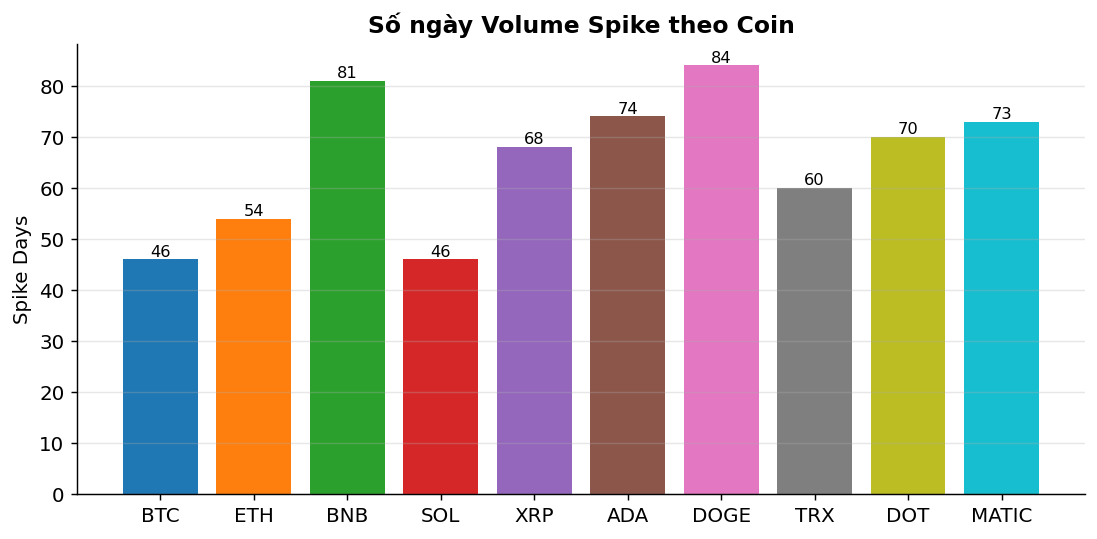
\includegraphics[width=0.85\linewidth]{Images/visualization/Is_Spike_Day.png}
    \caption{Số ngày Volume Spike theo coin}
    \label{fig:spike_count}
\end{figure}

Biểu đồ \ref{fig:spike_count} cho thấy số phiên Volume Spike trên 730 ngày của mỗi coin, dao động trong khoảng 50--80 phiên ($\sim$7--11\%). DOGE và XRP có số phiên spike cao hơn, phù hợp với đặc tính event-driven của hai mã này.

\textbf{Quy tắc giao dịch định lượng rút ra:}
\begin{itemize}
    \item \emph{Breakout xác nhận:} Một phiên có $return > +5\%$ chỉ được coi là tín hiệu phá vỡ đáng tin khi đi kèm Volume Spike.
    \item \emph{Breakdown xác nhận:} Tương tự với phiên giảm sâu $return < -5\%$.
    \item \emph{Feature dự báo:} Cờ \texttt{is\_spike} là feature có giá trị cao cho mô hình hồi quy/phân loại biến động.
\end{itemize}

\subsubsection{Heatmap tương quan và đồng biến động}

\begin{figure}[H]
    \centering
    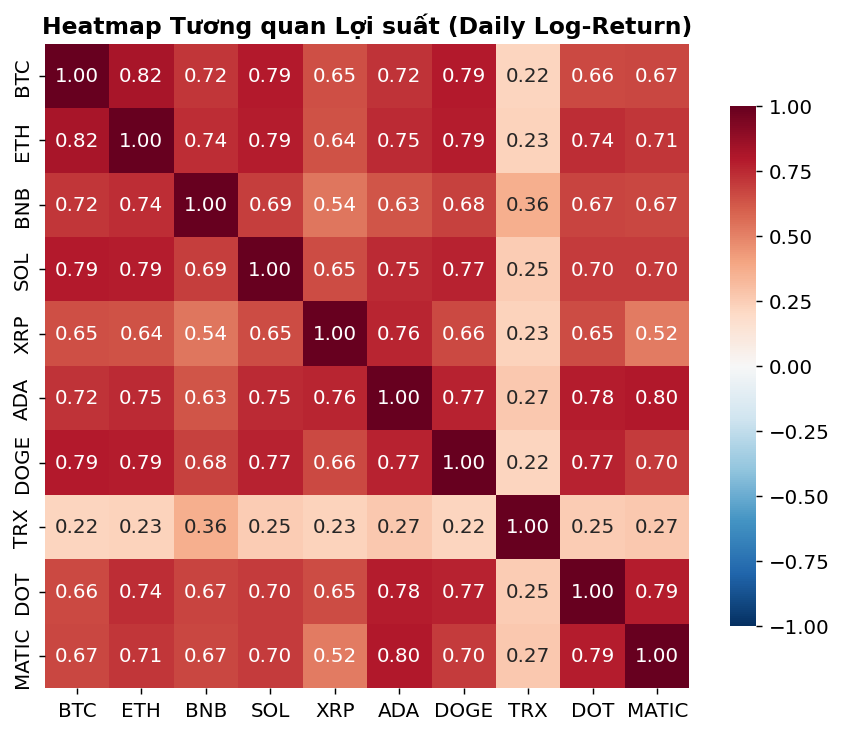
\includegraphics[width=0.95\linewidth]{Images/visualization/HeatmapLoiSuat.png}
    \caption{Heatmap tương quan log-return giữa 10 coin}
    \label{fig:heatmap_corr}
\end{figure}

Biểu đồ \ref{fig:heatmap_corr} thể hiện hệ số tương quan Pearson giữa các chuỗi log-return:
\begin{itemize}
    \item \textbf{Tương quan dương rất mạnh ($\rho > 0.8$):} Hầu hết các cặp altcoin Layer-1 (ETH--SOL, ETH--ADA, SOL--DOT, ...) cho thấy thị trường crypto vận động đồng pha cao -- khi BTC tăng, các altcoin đa phần cũng tăng theo.
    \item \textbf{BTC--altcoin ($\rho \approx 0.7-0.8$):} BTC đóng vai trò ``benchmark'' của toàn thị trường.
    \item \textbf{MATIC tách biệt:} Do dữ liệu chỉ đến 09/2024, tương quan với các coin khác thấp hơn rõ rệt.
\end{itemize}

\textbf{Hệ luận về đa dạng hoá} \cite{bodie2014}\textbf{:} Trong phạm vi 10 coin top, lợi ích đa dạng hoá nội bộ rất hạn chế -- gần như tất cả đều biến động cùng chiều. Để thực sự giảm rủi ro danh mục, nhà đầu tư cần kết hợp với các tài sản ngoài crypto (vàng, trái phiếu, cổ phiếu) -- nguyên lý Modern Portfolio Theory \cite{cfa2023}.

\begin{figure}[H]
    \centering
    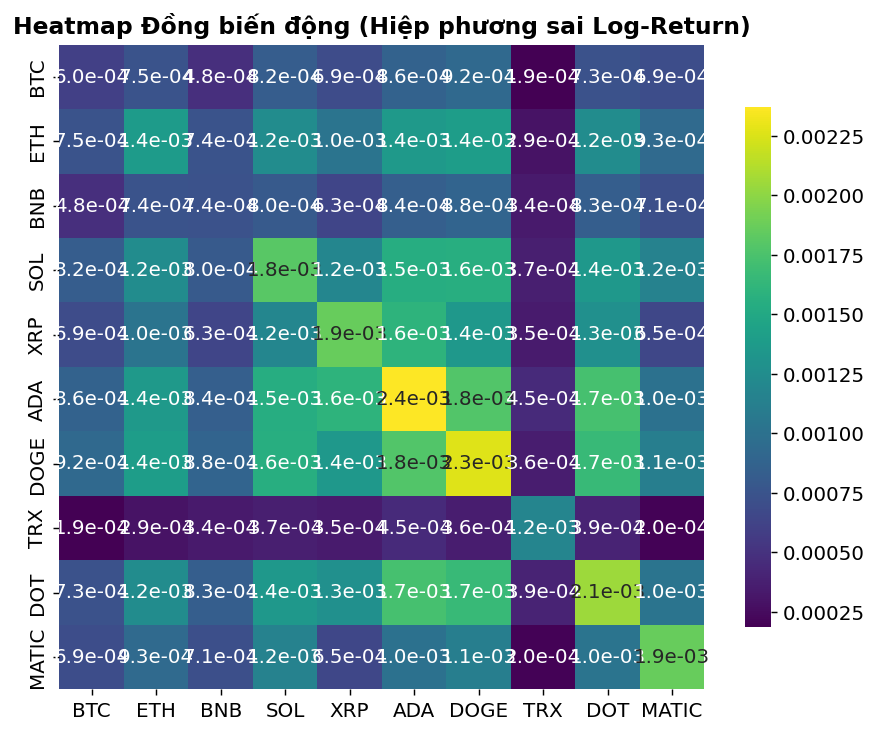
\includegraphics[width=0.95\linewidth]{Images/visualization/HeatmapDongBienDong.png}
    \caption{Heatmap đồng biến động (hiệp phương sai log-return)}
    \label{fig:heatmap_cov}
\end{figure}

Biểu đồ \ref{fig:heatmap_cov} thể hiện ma trận hiệp phương sai (covariance) -- khác với tương quan, các giá trị này phản ánh \emph{độ lớn thực tế} của biến động:
\begin{itemize}
    \item \textbf{Đường chéo (phương sai):} Cao nhất ở ADA, DOGE, DOT (rủi ro nội tại lớn). Thấp nhất ở BTC và TRX.
    \item \textbf{Ngoài đường chéo:} Tất cả đều dương cao, cho thấy rủi ro danh mục crypto khó giảm chỉ bằng cách đa dạng hoá nội ngành -- một hệ quả định lượng quan trọng cho việc xây dựng portfolio.
\end{itemize}

Hai heatmap này là \textbf{nền tảng toán học} cho thuật toán K-Means gom cụm: các coin có hiệp phương sai cao và cùng dấu sẽ được gom vào cùng cluster, tự động phân biệt nhóm low-vol vs high-vol mà không cần gắn nhãn thủ công.
